\documentclass[12pt, a4paper]{article}
\usepackage[utf8]{inputenc}
\usepackage{geometry}
\geometry{a4paper, margin=1.2in}
\usepackage{graphicx}
\usepackage{setspace}
\usepackage{hyperref}
\usepackage{tabularx}
\usepackage{float}
\usepackage{tikz}
\usepackage{booktabs}
\usepackage{pdflscape}

\doublespacing

\begin{document}

\begin{titlepage}
    \centering
    \vspace*{2cm}
    
    \Huge
    \textbf{Software Requirements Specification (SRS)}
    
    \vspace{0.5cm}
    \LARGE
    Project: Nucleus
    
    \vspace{1.5cm}
    
    \textbf{Continuous Behavioral Authentication and CI/CD Orchestration System}
    
    \vspace{2cm}
    
    \Large
    \textbf{Prepared by:} \\
    Shlok Burmi \\
    Yuvraj \\
    Sujal Kishore \\
    
    \vfill
    
    \Large
    \textbf{Date:} \today \\
    
\end{titlepage}

\tableofcontents
\newpage
\listoffigures
\newpage
\listoftables
\newpage

\section{Introduction}
\subsection{Purpose}
This Software Requirements Specification (SRS) provides a comprehensive description of the software requirements for the "Nucleus" project. Nucleus aims to establish a robust multi-service environment implementing continuous behavioral authentication utilizing LSTM models, coupled with an automated CI/CD pipeline using Jenkins and Docker. The primary objective is to enhance session security beyond traditional single-point authentication (such as OAuth and biometric checks) by continuously verifying user identity invisibly through interaction data.

\subsection{Document Conventions}
The following conventions have been followed in the preparation of this document:
\begin{itemize}
    \item \textbf{Bold text} is used to emphasize critical components or phases.
    \item \textbf{IEEE Standards:} This document conforms to the IEEE Std 830-1998 guidelines for Software Requirements Specifications.
    \item \textbf{Requirement Formatting:} Each distinct requirement is individually numbered for traceability.
\end{itemize}

\subsection{Intended Audience and Reading Suggestions}
This document is intended for project supervisors, system evaluators, software engineers, and testing engineers. It is recommended to review the overall system description before proceeding to the specific functional and non-functional requirements.

\subsection{Product Scope}
The Nucleus platform represents a significant advancement in identity verification for web applications. The software encompasses:
\begin{enumerate}
    \item A React-based front-end Dashboard interface.
    \item A robust Express/Node.js mapping backend integrated with MongoDB.
    \item Real-time Continuous Biometric Data collection (keystroke dynamics, mouse activity).
    \item An AI inference engine deploying Long Short-Term Memory (LSTM) machine learning models for anomaly detection and Imposter Simulation.
    \item Dynamic fallback mechanisms invoking step-up authentication (Face/Voice recognition).
    \item Seamless deployment through an automated Jenkins CI/CD pipeline.
\end{enumerate}

\subsection{References}
\begin{itemize}
    \item IEEE Guide to Software Requirements Specifications, ANSI/IEEE Std 830-1998.
    \item Nucleus JIRA Tracking Dashboard.
    \item Deep Learning in Continuous Authentication Research Papers.
\end{itemize}

\newpage
\section{Overall Description}
\subsection{Product Perspective}
The Nucleus system acts as an independent application managing its own decentralized ecosystem of microservices, linked securely through Docker networks. It provides the foundation of next-generation continuous verification for sensitive portals. It operates independently while relying on GitHub for version control and Jenkins for continuous delivery.

\subsection{Product Functions}
The principal functions of Nucleus are:
\begin{itemize}
    \item \textbf{OAuth Authentication:} Integration with Google Auth and GitHub Auth.
    \item \textbf{Behavioral Data Tracking:} Silent collection of interaction mechanics yielding raw vectors.
    \item \textbf{Continuous Inference:} Evaluation of live sessions against pre-trained LSTM architectures.
    \item \textbf{Adaptive Security:} Automated session invalidation or step-up factor (Face/Voice) requests upon threshold failures (High FAR/FRR events).
    \item \textbf{Automated Delivery:} Automatic linting, backend testing, Docker image building, and pushing to registries.
\end{itemize}

\subsection{User Classes and Characteristics}
\begin{enumerate}
    \item \textbf{End Students/Users:} Non-technical users accessing the Student Dashboard. Need transparent authentication mechanisms and high responsiveness.
    \item \textbf{System Administrators:} Technical personnel overseeing CI/CD health, ML model tuning (Hyperparameters), and manual overrides.
\end{enumerate}

\subsection{Operating Environment}
The software must operate gracefully within standard web browsers (Chrome, Firefox, Safari) and its backend infrastructure runs inside Docker containers orchestrated on Linux servers (or Windows Jenkins Agents substituting scripts accordingly).

\subsection{Design and Implementation Constraints}
\begin{itemize}
    \item Development constrained to MERN stack with external Python analytical modules.
    \item Latency of LSTM inference must not exceed 200ms to preserve UX.
    \item Jenkins pipelines must accommodate "Docker Desktop" interactions effectively, handling permissions precisely.
\end{itemize}

\newpage
\section{External Interface Requirements}
\subsection{User Interfaces}
The application employs a React front-end designed optimally for desktop environments, exhibiting material UI elements. 
\begin{itemize}
    \item \textbf{Dashboard Entry:} Features an intuitive login segment bridging Google and GitHub.
    \item \textbf{Verification Prompt:} A fallback modal requesting immediate voice passphrase or facial scan when anomalies are detected.
\end{itemize}

\subsection{Hardware Interfaces}
No designated exclusive hardware is necessary; standard human interface devices (mouse, keyboard) and media peripherals (webcam, microphone) are utilized to capture behaviors and biometrics.

\subsection{Software Interfaces}
\begin{itemize}
    \item \textbf{MongoDB Atlas:} Utilized for cloud-based or local scalable storage of behavioral vectors.
    \item \textbf{Jenkins Server API:} Utilized for monitoring build histories and triggering pipelines.
    \item \textbf{Docker CLI/Daemon:} Controls the instantiation of required images per build cycle.
\end{itemize}

\subsection{Communications Interfaces}
The system leverages:
\begin{itemize}
    \item HTTP/HTTPS for standard RESTful transactions.
    \item WebSockets for real-time streaming of behavioral matrices ensuring negligible buffering.
\end{itemize}

\newpage
\section{System Features and Use Cases}

\subsection{Multi-Factor Authentication Setup}
\textbf{Description:} Users must provision secondary authentication methods including Google/GitHub bindings and initial behavioral baseline accumulation.
\newline
\textbf{Flow:}
\begin{enumerate}
    \item User hits registration endpoint.
    \item User authorizes OAuth provision.
    \item Backend stores encrypted credentials and provisions a unique user identity.
\end{enumerate}

\subsection{Continuous Behavioral Authenticaton (LSTM)}
\textbf{Description:} Heart of the Nucleus project executing CAD-23 and CAD-25 milestones. A continuous tracking script gathers parameters.
\newline
\textbf{Flow:}
\begin{enumerate}
    \item Session Event occurs (MouseMove, KeyPress).
    \item Normalization pipeline scales metrics.
    \item Vector transmitted via WebSockets to Inference API.
    \item LSTM scores anomaly factor against registered user baseline.
\end{enumerate}

\subsection{Step-Up "Verification Needed" Fallback}
\textbf{Description:} Executes CAD-27 requirements. When confidence scores drop, the system intervenes.
\newline
\textbf{Flow:}
\begin{enumerate}
    \item System detects imposter probability exceeding threshold.
    \item UI freezes with "Verification Needed" dialog.
    \item Face/Voice validation processed.
\end{enumerate}

\subsection{CI/CD Automated Deployment Sequence}
\textbf{Description:} The Jenkins configuration orchestrating tests, builds, and service delivery.
\newline
\textbf{Flow:}
\begin{enumerate}
    \item Commit pushed to GitHub.
    \item Webhook triggers Jenkins master.
    \item Pipeline checks out source, executes npm tests.
    \item Success yields Docker build. Success yields Docker push to registry.
\end{enumerate}

\newpage
\section{Project Management and Agile Metrics}
We employed strict Agile methodology tracked via JIRA, and seamless CI/CD. The following metrics and visualizations outline our operational workflows and team contributions.

\subsection{Task Distribution and Timeline Analysis}
As seen from our milestone tracker, tasks were segregated intricately allowing robust component modularity.
\begin{figure}[H]
    \centering
    % Placeholder for first JIRA image
    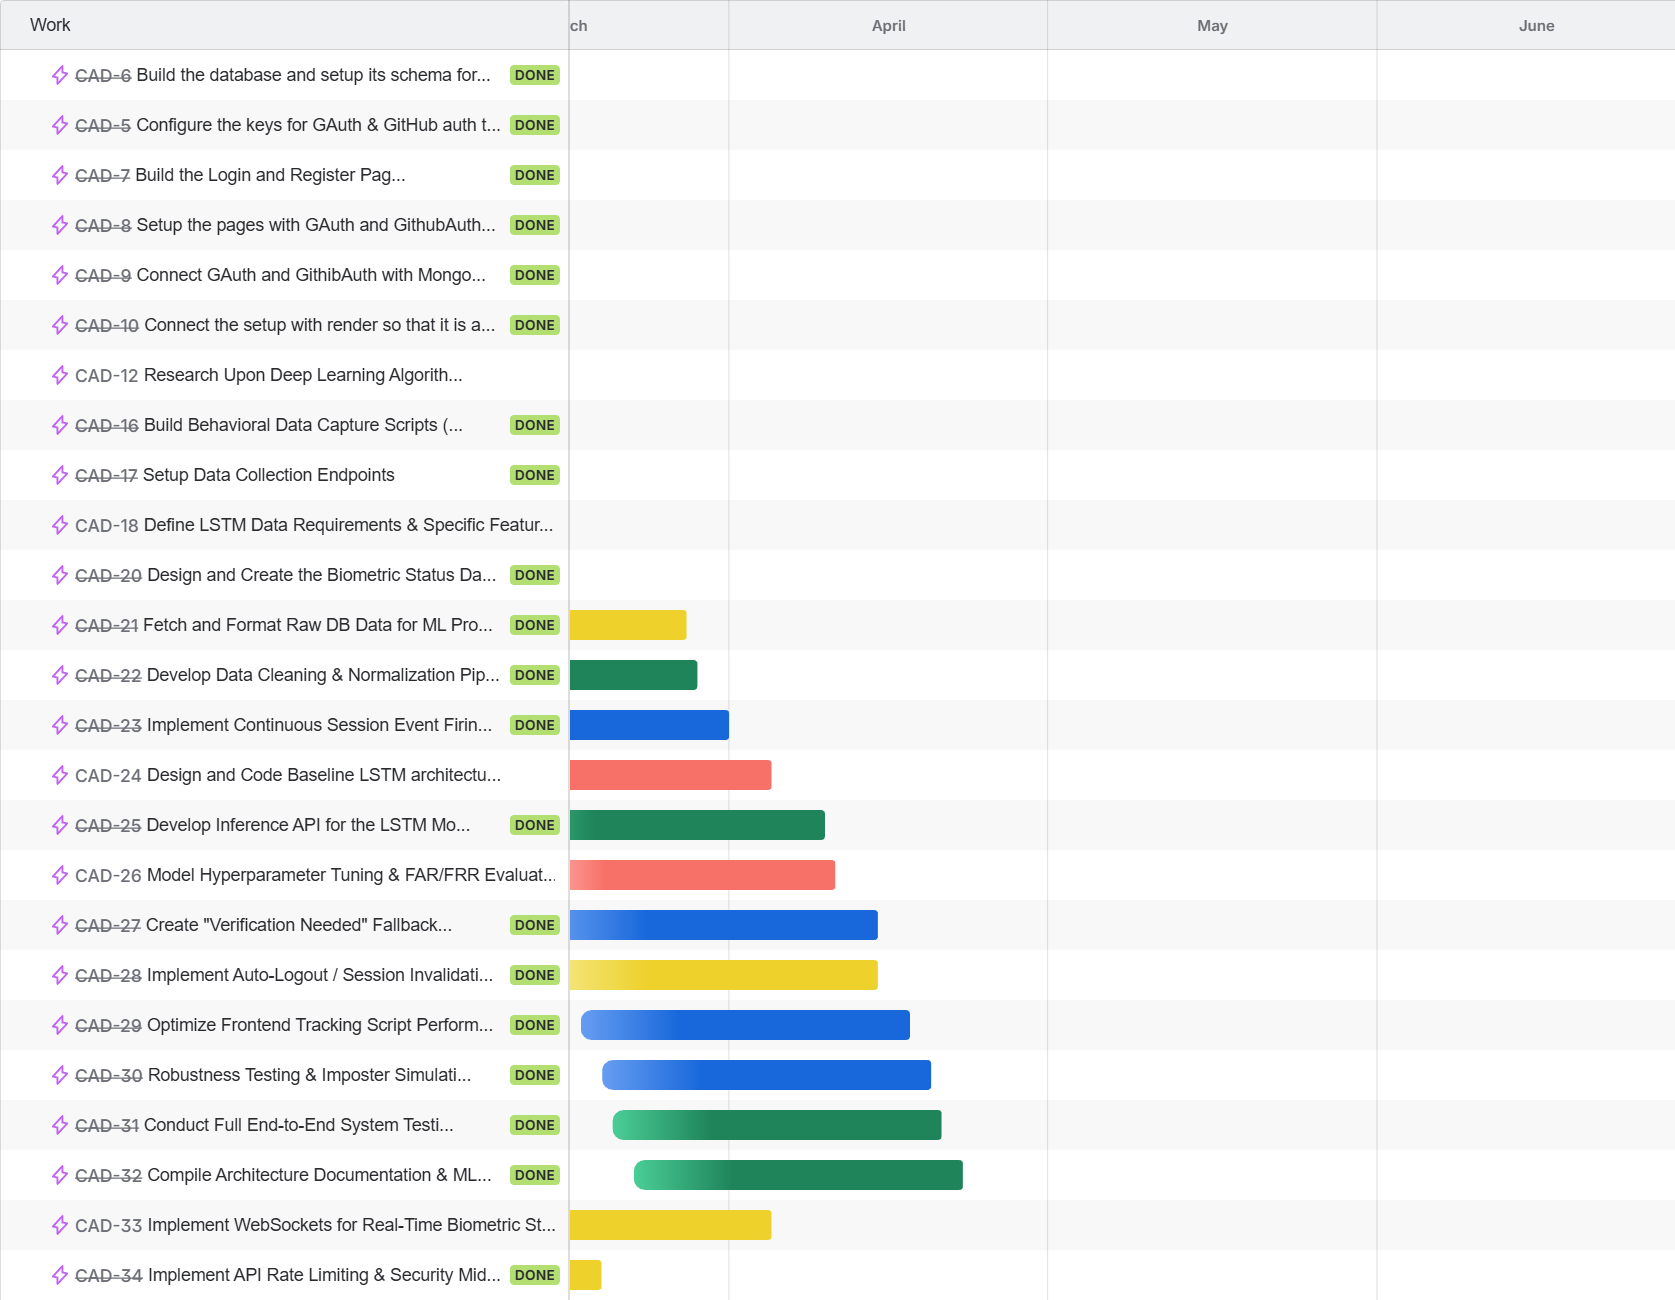
\includegraphics[width=0.9\textwidth]{jira.png}
    \caption{Nucleus JIRA Dashboard - Agile Sprints and Work Package Breakdown}
\end{figure}
As depicted in Figure 1, foundational phases including Database configuration (CAD-6) and OAuth implementations (CAD-5, CAD-7, CAD-8) were achieved smoothly. Subsequent phases required intensive research regarding LSTM design (CAD-24) and Continuous event firing mechanisms resulting in dynamic workflow adjustments.

\subsection{CI/CD Stage Profiling}
\begin{figure}[H]
    \centering
    % Placeholder for Jenkins image
    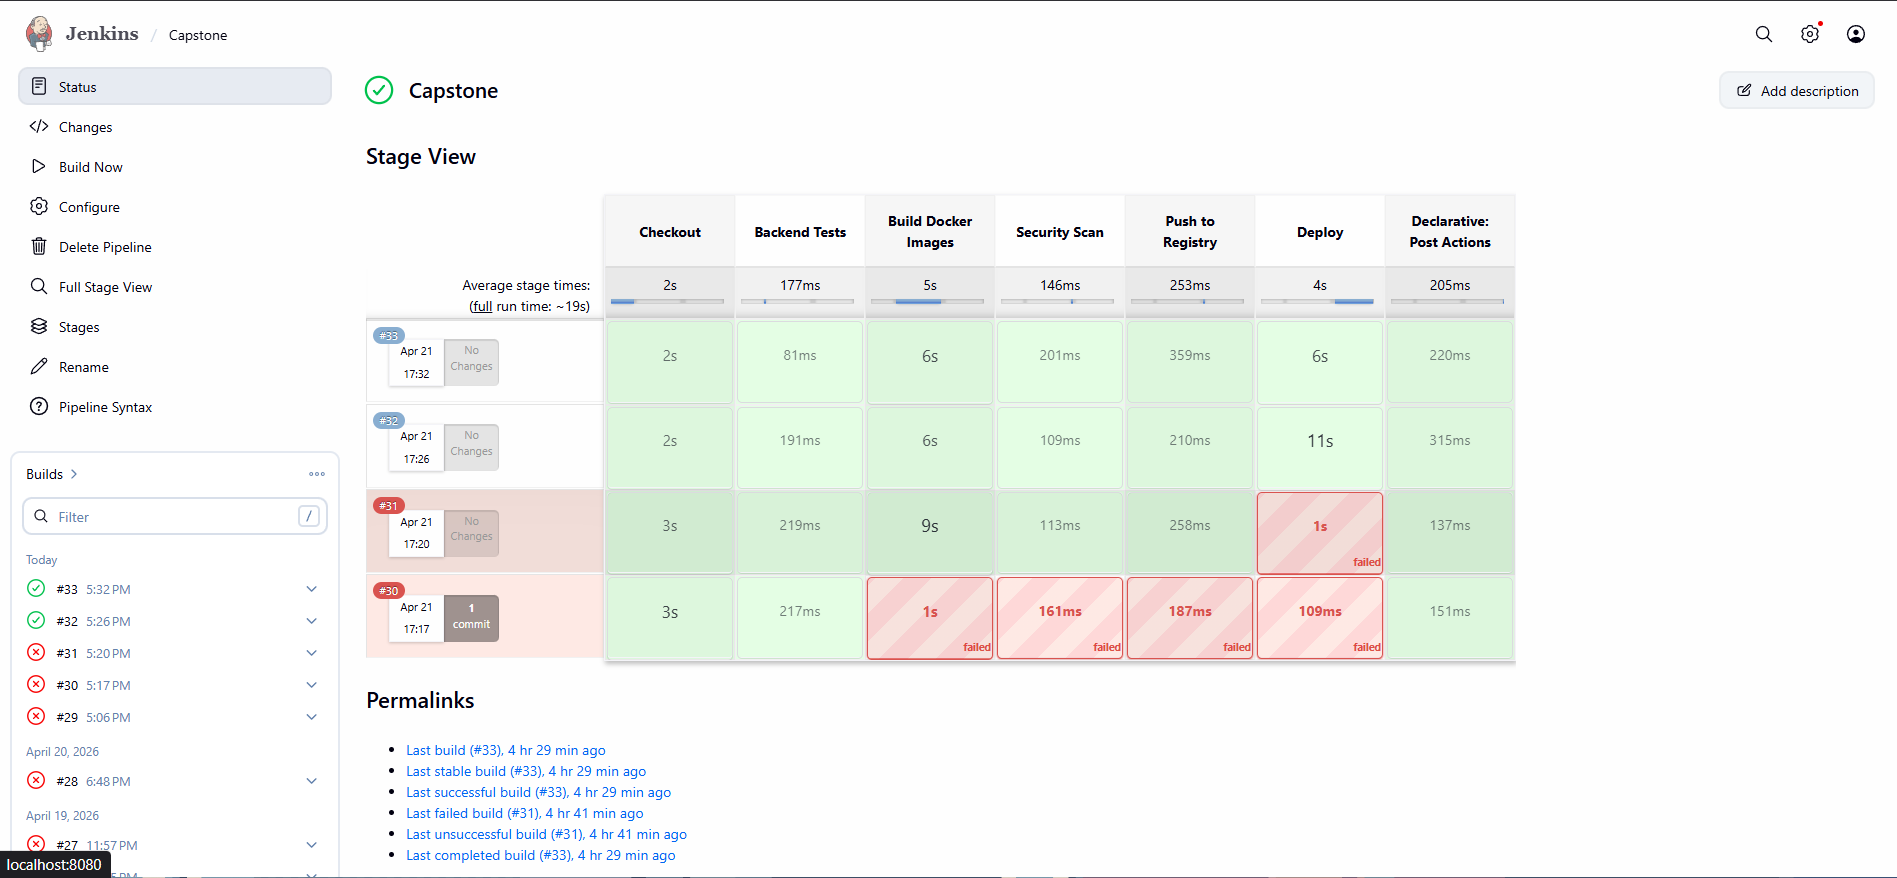
\includegraphics[width=1\textwidth]{jenkins.png}
    \caption{Jenkins Dashboard - Stage View Analysis (Capstone Pipeline)}
\end{figure}
Figure 2 illustrates the CI/CD Pipeline execution traversing multiple mandatory stages. From Code Checkout to Backend Testing (approx 177ms average), Docker Image Compilation, and Security Scans prior to deployment. The matrix visualizes test builds, explicitly logging failure margins for rapid patching cycles.

\newpage
\subsection{Repository Contributions and Code Kinetics}
\begin{figure}[H]
    \centering
    % Placeholder for third GitHub commits over time image
    \includegraphics[width=1\textwidth]{github_commits.png}
    \caption{GitHub Insights - Commits Frequency across Project Lifecycle}
\end{figure}
Figure 3 presents the commit timeline representing weekly sprint velocity and continuous integration patterns, ensuring no stagnation of code deployment. Peak iterations coincided with LSTM integration and pipeline stabilization.

\begin{figure}[H]
    \centering
    % Placeholder for fourth GitHub devs individual stats image
    \includegraphics[width=1\textwidth]{github_devs.png}
    \caption{GitHub Insights - Individual Developer Contributions}
\end{figure}
Figure 4 details individual impact analytics among core contributors (shlokburmi, yyyuvvvraj, SujalKishore). Over 13,000+ line insertions represent extensive framework implementations involving full-stack deployments and machine learning model configurations.

\newpage
\section{Non-Functional Requirements}

\subsection{Performance Requirements}
\begin{itemize}
    \item \textbf{Response Time:} Web pages must load effectively under 1.5 seconds.
    \item \textbf{Inference Engine:} Biometric validations must complete within milliseconds to avoid workflow interruption.
    \item \textbf{Throughput:} System must handle multiple concurrent WebSockets dynamically.
\end{itemize}

\subsection{Security Requirements}
\begin{itemize}
    \item Implementation of Rate Limiting \& Security Middleware as proposed in milestone CAD-34.
    \item Auto-logout controls to invalidate compromised sessions immediately.
    \item Secure storage for keys and secret constants out of version control arrays.
\end{itemize}

\subsection{Software Quality Attributes}
\begin{itemize}
    \item \textbf{Reliability:} Imposter simulations verify low False Acceptance Rates.
    \item \textbf{Maintainability:} Dockerized infrastructure allows modular component upgrades independently.
\end{itemize}

\newpage
\section{Appendix}
\subsection{Glossary}
\textbf{LSTM:} Long Short-Term Memory, an artificial recurrent neural network architecture. \\
\textbf{CI/CD:} Continuous Integration and Continuous Deployment. \\
\textbf{FAR:} False Acceptance Rate. \\
\textbf{FRR:} False Rejection Rate.

\end{document}
